\section{Distribution-based clustering\label{sec:distribution_based_clustering}}

\subsection{Method}

In Savoy (2014)'s \textit{Estimating the Probability of an Authorship Attribution}~\cite{savoy_probability} they modelled the true and false links score distribution using two Beta distribution.

As explained in~\cite{savoy_probability} the Beta distribution is better suited for authorship problem than, for example, the Gaussian distribution since it can grasp a larger amount of distribution shapes with its parameters flexibility.

In this study, we use these two models to find the position where the sum of the two areas under the curve is maximized.
It corresponds to the position in the rank list where the links true positive and true negatives are maximized according to the model (in a non-weighted minimization errors schema).
This position also correspond to where the two models have the same area under the curve and is called the equiprobable position.

Each Beta distribution require two parameters: $a$ and $b$.
Firstly to compute the parameters, the population must be normalized between 0 and 1 using Definition~\ref{def:normalization}.
The population are represented, for each distribution, by the true links or the false links scores.

\begin{definition}[Linear normalization \label{def:normalization}]
  Normalize a vector X in the interval $[0, 1]$.
  \begin{gather*}
    \begin{aligned}
      \alpha &= Min(X) \\
      \beta &= Max(X) - Min(X) \\
      Norm(X) &= \frac{X - \alpha}{\beta}
    \end{aligned}
  \end{gather*}
  Denormalize a scalar or a vector X from the interval $[0, 1]$ to the interval $[\alpha, \alpha + \beta]$
  \begin{gather*}
    DeNorm(X, \alpha, \beta) = X \cdot \beta + \alpha
  \end{gather*}
\end{definition}

The $a$ and $b$ parameters are estimated using the distribution population mean and the variance, see Definition~\ref{def:beta_parameters}

\begin{definition}[Beta distribution parameters \label{def:beta_parameters} \cite{savoy_probability}]
  \begin{gather*}
    \begin{aligned}
      \mu&: \mathrm{The\ population\ mean} \\
      \sigma&: \mathrm{The\ population\ standard\ deviation} \\
       \\
      \Delta &= \frac{\mu \cdot (1 - \mu)}{\sigma} - 1 \\
      a &= \mu \cdot \Delta \\
      b &= (1 - \mu) \cdot \Delta \\
    \end{aligned}
  \end{gather*}
\end{definition}

The Beta distribution probability density function (PDF) is computed using the formula in Definition~\ref{def:beta_pdf}

\begin{definition}[Beta distribution PDF \label{def:beta_pdf} \cite{savoy_probability}]
  \begin{gather*}
    \begin{aligned}
      Beta(X|a,b) = \frac{\Gamma(a + b)}{\Gamma(a) \cdot \Gamma(b)} \cdot X^{a-1} \cdot (1 - X)^{b-1}\\
      \mathrm{with\ }a > 0\mathrm{,\ }b > 0\mathrm{\ and\ }\Gamma()\mathrm{\ the\ Gamma\ function}
    \end{aligned}
  \end{gather*}
\end{definition}

The equiprobable position is found using a binary search between $0.00$ and $1.00$.
At each step, the cumulative distribution function (CDF) of the two Beta distribution are evaluated.
From left to right for the distribution on the left, and from right to left for the distribution on the right.
To compute this function, the scipy library is used.

Once the two area are obtained, their difference is computed.
The binary search stops once the difference is a small value, such as $10^{-15}$.
Binary searches have a complexity of $O(\log n)$.

There might be analytical ways to solve this problematic using the \textit{Beta distribution cumulative distribution function analytic form} (Beta CDF analytic form) but was out of the scope of this study.
With an analytical solve, the complexity could drop to $O(1)$.

Figure~\ref{fig:links_score_density} shows the distance density for true and false link as well as a Beta distribution estimation for the St-Jean B rank list generated with text representation 0 (ref. Section~\ref{sec:individual_methods_summary}).

The vertical line in this figure, indicates the equiprobable position where both Beta distribution have the same probability of being a true link and false link (same area under the curve).
This point can be used as a decision point where the cut should be made in the rank list, this ensures that both false positives and false negatives are minimized.

Once the equiprobable position is found for a corpus with known authors, it can be re-used for new corpora.
After denormalizing (see Definition~\ref{def:normalization}), the equiprobable position is used as a distance threshold to stop the hierarchical clustering.

This method is supervised, since it requires examples to learn the cut.
The distribution-based clustering do not consider any new corpus for its value computation.
Each training rank list yields a single fixed real number, the optimal cut position for this rank list.

\begin{figure}[!t]
  \caption{Links distances density and Beta distribution estimation for St-Jean B with text representation 0}
  \label{fig:links_score_density}
  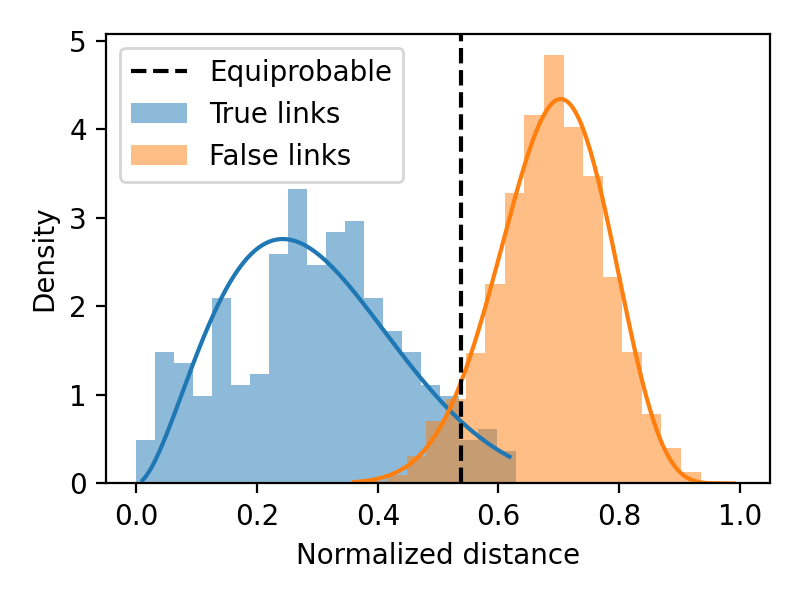
\includegraphics[width=\linewidth]{img/links_score_density.png}
\end{figure}

\subsection{Possible Cost Function}

This technique can be adapted, in the case where a loss/cost function have to be minimized.
This can be used when the false positives do not have the same importance as false negatives.

To introduce a cost function to the two Beta method, the position search criterion is changed.
Instead of finding the position where both the true link and false link area correspond to $50\%$ of their sum (equiprobable case).
We can aim to find where true links area correspond to, for example, $60\%$ and false links area to $40\%$ in this case.

It can be generalized such that the true link area represent $\alpha$ and the false link area to $1-\alpha$ with $\alpha \in \left[0,1\right]$.
When $\alpha$ is greater than $0.50$, more false positives and less false negatives will occur.
When $\alpha$ is smaller than $0.50$, less false positives and more false negatives will occur.

For the clustering, the $\alpha$ parameter directly influence the $r_diff$ value and the $B^3_{precision}$ and $B^3_{recall}$.
The same binary search can be used for this computation, just the target need to be changed.
In this study, we only considered the equiprobable case for the experiments.

\subsection{Evaluation}

The distribution-based clustering approach is evaluated using the Oxquarry, Brunet, St-Jean A and B corpora.
The retained rank list for each corpus used are in Annex (Table~\ref{tab:rls_oxquarry_brunet} and Table~\ref{tab:rls_st_jean}).
For each rank list, the distance threshold is computed using the two Beta approach.
This step corresponds to the training phase.

Then for every distance threshold and rank list pair, the hierarchical clustering is applied.
This corresponds to the testing phase.
The results are evaluated using the $B^3_{F_1}$ and the $r_{diff}$ metrics.
The evaluation results are aggregated by applying the arithmetic mean on the $B^3_{F_1}$ and $r_{diff}$ across all retained rank list.

The evaluation is presented in Table~\ref{tab:semi_supervised_clustering} which show the results for each linkage criterion (Single, Average, Complete).

The following conclusions can be drawn with these results:
\begin{itemize}
  \item
  In terms of linkage criteria, the single linkage is not adapted, with an average $B^3_{F_1} = 0.22$.
  \item
  Average linkage have the best $r_{diff} = 0.06$ which indicate that this criterion can estimate the most accurately the number of clusters.
  \item
  Complete linkage have the best $B^3_{F_1} = 0.82$ which make it the best criterion for this method. Which is $8\%$ better than the average linkage and $273\%$ better than the single linkage.
  \item
  The training corpus does not influence a lot the quality of the results.

  $std(\mathrm{MeanTraining}_{B^3_{F_1}}) = 0.01$

  The best corpus to train is Brunet, with slightly better results.
  \item
  In the other hand, the quality of the rank list used for the testing phase is more impactful.

  $std(\mathrm{MeanTesting}_{B^3_{F_1}}) = 0.04$

  This further validate the assumption made in Section~\ref{sec:hierarchical_clustering}.
  St-Jean B's rank list have the best average precision and the best clustering results.
\end{itemize}

\begin{table*}[!t]
  \centering
  \caption{Distribution-based clustering evaluation, mean $B^{3}_{F_1}$/$r_{diff}$ for each corpus pair}
  \label{tab:semi_supervised_clustering}

  \subcaption{Single Linkage}
  \begin{tabular}{l l| c c c c|c}
    \toprule
    \multicolumn{2}{c}{\multirow{2}{*}{}} & \multicolumn{4}{c}{Testing} \\
    \multicolumn{2}{c}{} & Oxquarry & Brunet & St-Jean A & St-Jean B & Mean \\
    \midrule
    \parbox[!t]{2mm}{\multirow{4}{*}{\rotatebox[origin=c]{90}{Training}}}
    & Oxquarry  & 0.27/0.15 & 0.18/0.22 & 0.14/0.16 & 0.12/0.18 & 0.18/0.18\\
    & Brunet    & 0.36/0.12 & 0.18/0.22 & 0.15/0.16 & 0.12/0.18 & 0.20/0.17\\
    & St-Jean A & 0.42/0.11 & 0.30/0.19 & 0.14/0.16 & 0.13/0.18 & 0.25/0.16\\
    & St-Jean B & 0.42/0.10 & 0.35/0.16 & 0.16/0.16 & 0.16/0.17 & 0.27/0.15\\
    \midrule
    & Mean      & 0.37/0.12 & 0.25/0.20 & 0.15/0.16 & 0.13/0.18 & 0.22/0.16\\
    \bottomrule
  \end{tabular}

  \vspace{0.5cm}

  \subcaption{Average Linkage}
  \begin{tabular}{l l| c c c c|c}
    \toprule
    \multicolumn{2}{c}{\multirow{2}{*}{}} & \multicolumn{4}{c}{Testing} \\
    \multicolumn{2}{c}{} & Oxquarry & Brunet & St-Jean A & St-Jean B & Mean \\
    \midrule
    \parbox[!t]{2mm}{\multirow{4}{*}{\rotatebox[origin=c]{90}{Training}}}
    & Oxquarry  & 0.73/0.04 & 0.65/0.08 & 0.59/0.10 & 0.61/0.11 & 0.65/0.08 \\
    & Brunet    & 0.78/0.05 & 0.73/0.04 & 0.73/0.07 & 0.73/0.08 & 0.74/0.06 \\
    & St-Jean A & 0.82/0.05 & 0.74/0.06 & 0.81/0.04 & 0.83/0.05 & 0.80/0.05 \\
    & St-Jean B & 0.83/0.09 & 0.79/0.08 & 0.83/0.02 & 0.90/0.02 & 0.84/0.05 \\
    \midrule
    & Mean      & 0.79/0.06 & 0.73/0.06 & 0.74/0.06 & 0.77/0.06 & 0.76/0.06 \\
    \bottomrule
  \end{tabular}

  \vspace{0.5cm}

  \subcaption{Complete Linkage}
  \begin{tabular}{l l| c c c c|c}
    \toprule
    \multicolumn{2}{c}{\multirow{2}{*}{}} & \multicolumn{4}{c}{Testing} \\
    \multicolumn{2}{c}{} & Oxquarry & Brunet & St-Jean A & St-Jean B & Mean \\
    \midrule
    \parbox[!t]{2mm}{\multirow{4}{*}{\rotatebox[origin=c]{90}{Training}}}
    & Oxquarry  & 0.79/0.06 & 0.77/0.05 & 0.82/0.04 & 0.84/0.04 & 0.81/0.05 \\
    & Brunet    & 0.79/0.10 & 0.81/0.09 & 0.84/0.02 & 0.90/0.02 & 0.83/0.06 \\
    & St-Jean A & 0.79/0.11 & 0.81/0.11 & 0.82/0.05 & 0.90/0.02 & 0.83/0.07 \\
    & St-Jean B & 0.78/0.13 & 0.79/0.14 & 0.77/0.09 & 0.90/0.04 & 0.81/0.10 \\
    \midrule
    & Mean      & 0.79/0.10 & 0.80/0.10 & 0.81/0.05 & 0.88/0.03 & 0.82/0.07 \\
    \bottomrule
  \end{tabular}

\end{table*}
